\section{System Design and Experimental Setup}
\label{sec:system-design}
\label{sec:setup}

The IPI protocol supports stateless CV/ITS applications and stateful CAV
applications. We use workload sizes and directions representative of both
communication patterns to compare direct PC5 and network-assisted Uu. We
measure response RTT and deadline completion for each workload. The
exact directional transfers additionally measure receiver-observed application
goodput after byte-count and checksum validation. The
study covers the two access modes emphasized by the 3GPP V2X architecture:
direct PC5 communication and network-assisted Uu communication
\cite{etsi123287r18}. PC5 exchanges data locally between vehicles and roadside
infrastructure. Uu carries vehicle traffic through a radio access network and
mobile core to an application endpoint. The experiments use one
commercial implementation of each path on the same autonomous vehicle.
Protocol fields and serialization additions are reported in bytes (B).
Application payloads and transferred objects use kibibytes
($\mathrm{KiB}=2^{10}$~B) or mebibytes ($\mathrm{MiB}=2^{20}$~B). Link rates
and application goodput use decimal kilobits per second (kbit/s), megabits per
second (Mbit/s), or gigabits per second (Gbit/s).

\subsection{Testbed and Measured Paths}

Figure~\ref{fig:testbed-overview} presents the testbed topology and equipment.
The vehicle host runs the workload sender and sender-side timer. Its
PC5 interface is a Mocar on-board unit (OBU), and its Uu interface is an MG52 or
GL-X3000 gateway. The corresponding radio endpoints are a fixed HUALI roadside
unit (RSU) and an outdoor Airspan AirSpeed 2900 gNodeB. Both paths terminate at
the d1 application host, which connects directly to the RSU and the on-site
MX250. The remote MX68CW manages the private 5G deployment and is outside the
measured user-data path~\cite{cisco2025private5g,cisco2026mx250,cisco2026mx68}.

\begin{figure*}[t]
  \centering
  \begin{tikzpicture}[
      font=\small,
      >={Stealth[length=2.2mm]},
      node/.style={draw, rounded corners=2pt, align=center, minimum height=0.78cm,
                   inner sep=3pt, text width=1.75cm},
      host/.style={node, text width=2.35cm},
      link/.style={<->, line width=0.8pt}]
    \node[host, fill=blue!5] (host) at (-6.5,0)
      {Vehicle host\\sender and timer};
    \node[node, fill=blue!5] (obu) at (-3.5,1.0) {Mocar OBU};
    \node[node, fill=blue!5] (mg52) at (-3.5,-1.0) {5G gateway\\MG52 or GL-X3000};
    \node[node, fill=green!7] (rsu) at (0,1.0) {HUALI RSU};
    \node[node, fill=green!7] (ran) at (-0.4,-1.0) {n48 gNodeB};
    \node[node, fill=green!7] (core) at (2.4,-1.0) {Private 5G};
    \node[node, fill=green!7] (mx) at (4.8,-1.0) {MX250};
    \node[host, fill=orange!8] (endpoint) at (7.2,0)
      {d1 host\\workload responder};
    \draw[->,line width=0.8pt] (host.north east) -- (obu.west);
    \draw[link] (obu) -- node[above] {PC5} (rsu);
    \draw[link] (rsu) -- (endpoint);
    \draw[->,line width=0.8pt] (host.south east) -- (mg52.west);
    \draw[link] (mg52) -- node[above] {NR Uu} (ran);
    \draw[link] (ran) -- (core);
    \draw[link] (core) -- (mx);
    \draw[link] (mx) -- (endpoint);
  \end{tikzpicture}
  \caption{Testbed and equipment overview. The autonomous-vehicle host reaches
  d1 through either the commercial Mocar/HUALI PC5 equipment or the
  MG52/GL-X3000, n48 gNodeB, private-5G, and MX250 Uu equipment. The two paths
  share the vehicle host and d1 endpoint but were measured separately.}
  \Description{An autonomous-vehicle host connects through an on-board unit and
  roadside unit over PC5 or through a cellular gateway, n48 gNodeB, private 5G
  system, and local MX250 over Uu. Both paths terminate at the directly
  connected d1 workload responder.}
  \label{fig:testbed-overview}
\end{figure*}

The PC5 equipment uses the vendor's 2020 J2735 stack. We first exercised its
standard-message callbacks. The performance probes then used the vendor's
packet-data interface with a sequence number and same-size echoed payload. The
installed interface accepts application packets up to 4,080~B, and the
evaluated sweep uses 0--2~KiB. The vendor reports protocol-conformance
certification for the product families~\cite{huali2021certification}.

Most Uu campaigns connect the vehicle host to a Cisco Meraki MG52 gateway over
1-Gbit/s Ethernet. The MG52 contains the subscriber identity module (SIM) and
an internal antenna placed face-up on the trunk floor. The August 19
directional repeat replaces the MG52 with a GL.iNet GL-X3000 gateway and
evaluates both TDD configurations with that device. Each gateway reaches d1
through the AirSpeed gNodeB, the Cisco private 5G system, and the on-site MX250.

Figure~\ref{fig:measurement-paths} expands these components into the measured
request and response paths. A PC5 request returns a sequence-matched,
same-size echo. The Uu probes carry IPI Cooperative Service frames. In an
uplink-heavy exchange, the vehicle sends the declared application object, and
d1 returns a compact correlated acknowledgment after decoding it. In a
downlink-heavy exchange, the vehicle sends a compact request, and d1 returns
the requested application object. The vehicle validates the response sequence
number, length, and checksum before stopping its RTT timer.

\begin{figure*}[t]
  \centering
  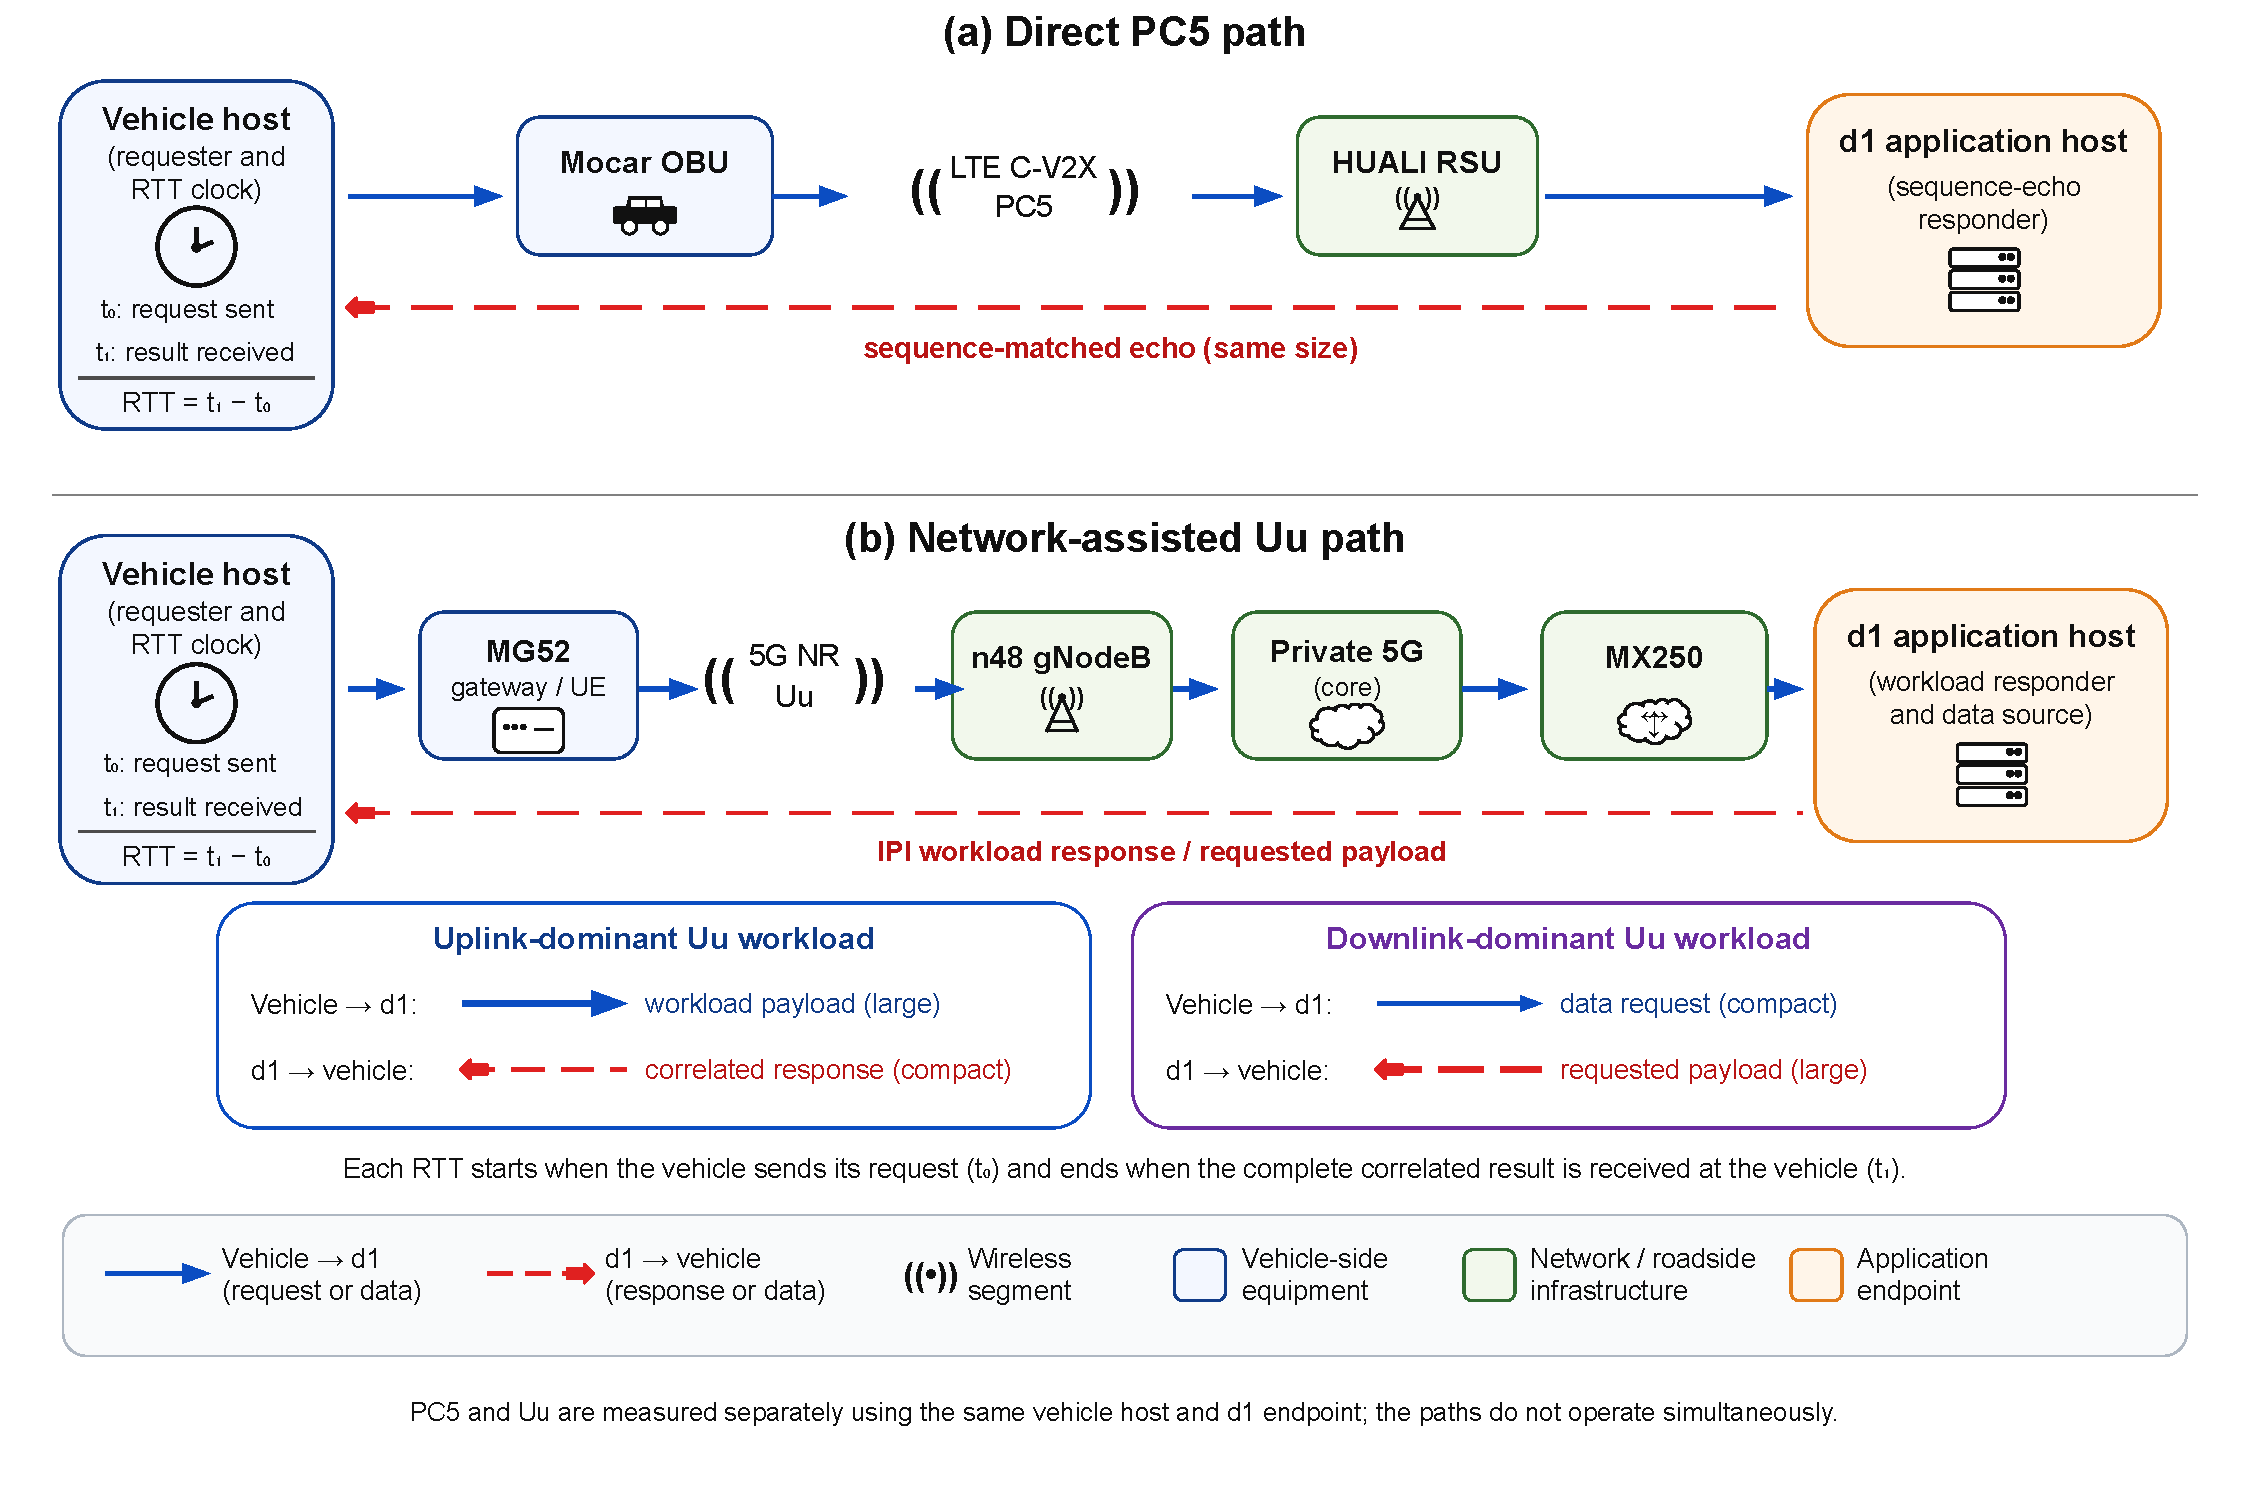
\includegraphics[width=\textwidth]{../figs/edge4av_figure3_editable.pptx.pdf}
  \caption{Detailed request/response data paths and sender-side RTT boundaries.
  (a) The direct PC5 request returns a same-size, sequence-matched echo. (b) The
  network-assisted Uu path carries either a large vehicle-originated IPI
  workload followed by a compact correlated response or a compact vehicle
  request followed by the complete requested payload. PC5 and Uu were measured
  separately.}
  \Description{Two panels expand the testbed overview into detailed data paths.
  The PC5 panel shows a vehicle request and same-size sequence echo through the
  on-board and roadside units. The Uu panel shows uplink-heavy and
  downlink-heavy IPI exchanges through the gateway, gNodeB, private 5G system,
  MX250, and d1, together with the sender-side round-trip timing boundary.}
  \label{fig:measurement-paths}
\end{figure*}

The Uu deployment was tightly controlled. The vehicle gateway was the sole user
equipment (UE), and the AirSpeed radio and its full 40-MHz channel were
dedicated to the experiment. The Citizens Broadband Radio Service (CBRS) n48
band was clean and carried no ambient traffic. The baseline measurements
contained no unrelated user devices or ambient radio-band contention.
Background streams and 1--100 application clients were introduced only as
controlled experimental variables behind the same UE attachment.
Table~\ref{tab:deployment} summarizes the controls that bound the application
measurements and identifies the comparison enabled by each control.

\begin{table*}[t]
  \caption{Experimental controls and their roles in the analysis.}
  \label{tab:deployment}
  \centering
  \footnotesize
  \setlength{\tabcolsep}{4pt}
  \renewcommand{\arraystretch}{1.12}
  \begin{tabular}{@{}C{0.15\textwidth}C{0.36\textwidth}C{0.41\textwidth}@{}}
    \toprule
    Dimension & Controlled condition & Role in comparison \\
    \midrule
    Radio occupancy & Dedicated 40-MHz n48 channel; no ambient users or traffic & Establishes the single-UE baseline; load is introduced only by the experiment \\
    Client population & One physical CAV UE; 1--100 logical clients share its attachment & Varies application concurrency without changing the number of radio clients \\
    Endpoint and timing & d1 directly connected to the RSU and MX250; unsynchronized endpoint clocks & Measures sender-side RTT and validated goodput; does not infer one-way delay \\
    Field context & Stationary workload records; continuous-drive RSRP/SINR survey; GNSS-joined PC5 outcomes & Relates application measurements to stationary conditions and route coverage \\
    Configuration and gateway & 70/20/10 and 40/40/20; MG52 and GL-X3000 repeats & Tests whether TDD behavior persists across vehicle gateways and both traffic directions \\
    \bottomrule
  \end{tabular}
\end{table*}

The 5G radio uses 30-kHz subcarrier spacing and TDD. The operator reported
70/20/10 as the deployment's established allocation. These values denote the
downlink, uplink, and dynamic shares. All application campaigns before the TDD
study used this profile. Its downlink-oriented allocation is consistent with
the downlink-heavy frame structures reported for current 5G deployments
\cite{ngmn2021tdd}. We also evaluate 40/40/20, which assigns 40\% of the frame
to fixed uplink use rather than 20\%. Both profiles retain 10D4G frame packing.
The TDD study includes repeated uplink-heavy RTT sweeps, matched downlink-heavy
RTT sweeps, and exact 50-MiB transfers in each direction. A replacement-gateway
repeat uses the GL-X3000 for complete uplink-heavy and downlink-heavy matrices
and three exact transfers per direction under each profile. Each run
records the application direction, location, and available signal context;
the earlier runs additionally record available cell state and serving-cell
context.
The Airspan distributed-unit (DU) Cell exports provide five-minute cell volume,
active-time, and unavailability counters for the available windows. These
counters verify the serving cell and measurement-block context. Endpoint
records define application RTT and goodput.

A Samsung 22 handset running G-NetTrack Pro recorded radio conditions during
three continuous drives through the testbed. The combined trace contains
1,301 Global Navigation Satellite System (GNSS) records. We remove 123 records
from a frozen radio-value interval longer than 5~s and retain 1,178 valid New
Radio (NR) band-48 records. Reference Signal Received Power (RSRP) spans
$-121$ to $-88$~dBm, with a median of $-108$~dBm. The corresponding NR
signal-to-interference-plus-noise ratio (SINR) spans $-20$ to 30~dB, with a
median of 9~dB. G-NetTrack Pro's ordinary signal-to-noise ratio field is empty.
We recover SINR from the timestamped NR \texttt{ssSinr} entries in the verbose
logs and align each entry to its nearest GNSS record.

3GPP defines the 5G Synchronization Signal Reference Signal Received Power
(SS-RSRP) measurement but does not assign qualitative coverage levels
\cite{etsi138215r19}. We aggregate the outdoor pedestrian levels in
Australia's 2026 coverage-map standard \cite{acma2026coverage}: Good maps to
strong ($\mathrm{RSRP}\geq -95$~dBm), Moderate maps to common/typical
($-105\leq\mathrm{RSRP}<-95$~dBm), and Basic and No Coverage map to weak
($\mathrm{RSRP}<-105$~dBm).

The temporal sample distribution contains 83 (7.0\%) strong, 340 (28.9\%)
common/typical, and 755 (64.1\%) weak records. We use the drive survey to
characterize route-level coverage and each workload campaign's signal record
to compare stationary application measurements.
Figure~\ref{fig:signal-survey} maps local interpolation of RSRP and SINR within
the sampled boundary. The PC5 route analysis joins every issued request and
received response to GNSS coordinates, producing spatial response-completion
and RTT measurements along each driven path.

\begin{figure*}[t]
  \centering
  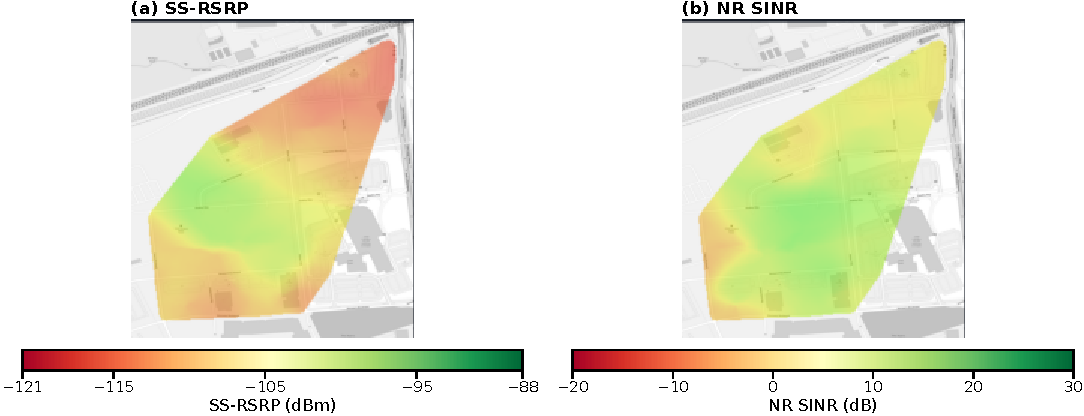
\includegraphics[width=0.88\textwidth]{figures/section4_signal_survey.pdf}
  \caption{Continuous-drive radio survey of the private 5G testbed. A Samsung 22
  handset running G-NetTrack Pro recorded three drive segments. The maps
  interpolate (a) SS-RSRP and (b) recovered NR SINR from 1,178 valid band-48
  records within the sampled boundary. Records from a frozen radio-value
  interval longer than 5~s are excluded. Map data © OpenStreetMap contributors.}
  \Description{Two OpenStreetMap panels show interpolated RSRP and recovered
  New Radio signal-to-interference-plus-noise ratio from three continuous drive
  segments recorded by a Samsung 22 handset running G-NetTrack Pro.}
  \label{fig:signal-survey}
\end{figure*}

Figure~\ref{fig:measurement-paths} defines the request and response events at
the RTT boundary. The PC5 RTT covers the vendor
interface, two direct-radio traversals, response handling, and correlation. The
Uu RTT covers the vehicle host, gateway, radio access, private core, local
routing, d1 responder, and return path. The d1
responder decodes each workload frame and immediately returns its response.
Its direct connections to the RSU and MX250 make local wired transfer
negligible relative to the measured communication paths. The clocks were not
synchronized, so all timing uses the sender's round-trip clock. Each timer
begins immediately before the vehicle transmits its request. An uplink-heavy
timer ends when the vehicle receives the compact acknowledgment. A
downlink-heavy timer ends after the vehicle receives and validates the complete
requested payload.
The exact 50-MiB transfer experiment uses a separate endpoint timer. The
receiver verifies the payload size and checksum before reporting the
transfer duration and application goodput.

\subsection{Application Conditions and Workloads}

Connected-vehicle and CAV applications place different data sizes, dominant
directions, durations, and deadlines on the communication path.
Table~\ref{tab:application-envelopes} maps six representative applications to
the workload probes used to evaluate these requirements
\cite{nhtsa2005vsc,etsi122186r19,fivegaa2021usecases,he2024transformative}.
Periodic signal and collision warnings create compact shared updates. For
emergency-vehicle signal priority, an authorized vehicle sends an SRM to
request priority or preemption, and the infrastructure returns the request
status in an SSM~\cite{saej2735_2024}. Remote assistance for a disabled or
malfunctioning CAV can begin with a compact request and return perception,
planning, control, or other data from an edge or help-center endpoint. Remote
recovery can also add a continuous vehicle-originated video stream. At
25~mph, the vehicle moves 0.11~m in 10~ms and 1.12~m in 100~ms. Under Federal
Highway Administration assumptions, its level-road stopping sight distance is
about 46.3~m~\cite{fhwa2009speed}. A 35-mph adjacent vehicle changes its gap to
a 25-mph vehicle by 0.45~m in 100~ms. Remote assistance below 10~km/h moves a
vehicle at most 0.278~m in 100~ms and 0.556~m in 200~ms. These applications
cannot be represented by one payload, direction, duration, or deadline.
Their traffic can be periodic, event triggered, or continuous. Perception,
intent, and fault state create vehicle-to-edge demand. A compact vehicle
request can instead return raw sensor data, processed perception, planning
data, control data, or other state from the edge. Several operations can also
share the same attachment while a continuing stream remains active.

\begin{table*}[t]
  \caption{Representative application requirements and workload probes.
  $\uparrow$ denotes vehicle-to-edge traffic and $\downarrow$ denotes
  edge-to-vehicle traffic. Object sizes exclude transport and security bytes.}
  \label{tab:application-envelopes}
  \centering
  \footnotesize
  \setlength{\tabcolsep}{2.5pt}
  \renewcommand{\arraystretch}{1.15}
  \begin{tabular}{@{}C{0.17\textwidth}C{0.20\textwidth}C{0.18\textwidth}C{0.11\textwidth}C{0.24\textwidth}@{}}
    \toprule
    Application & Traffic pattern & Object size or rate & Deadline & Workload probe \\
    \midrule
    Signal phase/status & Periodic infrastructure $\downarrow$ & About 0.5~KiB at 10~Hz & 100~ms & SPaT callback; compact PC5/Uu cycles \\
    Collision or blind-spot warning & Periodic many-to-many PC5 & About 0.2~KiB per source at 10~Hz & 100~ms & 0.25-KiB stationary and route PC5 cycles \\
    Emergency-vehicle signal priority & SRM $\uparrow$; SSM $\downarrow$ & 0.3--1~KiB & 10~ms & SRM/SSM callbacks; 0.25--1-KiB cycles \\
    Emergency maneuver & Reciprocal event-triggered burst $\uparrow\downarrow$ & 2--12~KiB & 3--10~ms & 2-KiB PC5; 8--16-KiB Uu cycles \\
    Remote-assistance data request & Compact request $\uparrow$; application object $\downarrow$ & 1--500~KiB & 100--1,000~ms & Downlink-heavy TCP/MQTT cycles \\
    Fault-triggered remote recovery & Video/state $\uparrow$; control/path $\downarrow$ & Up to 1~KiB control; 32-Mbit/s video & 100/200~ms & Bidirectional Uu; exact transfer, load, demand, and restart \\
    \bottomrule
  \end{tabular}
\end{table*}

The application conditions define four parts of the workload matrix:
\begin{enumerate}
  \renewcommand{\labelenumi}{\arabic{enumi})}
  \item \textbf{Payload and direction.} PC5 spans 0--2~KiB. Uu spans
  0--2~MiB using a vehicle-originated object followed by a compact
  acknowledgment. The downlink-heavy probe returns an exact 1-, 10-, 100-, or
  500-KiB object after a compact vehicle request. Separate 50-MiB transfers
  measure validated goodput in each direction.
  \item \textbf{Application-object size.} The Uu sweep includes 922 V2X-Radar
  object lists: 19.2~KiB at the median, 23.4~KiB at the 99th percentile, and
  24.4~KiB at the maximum. Additional dataset objects span 8~KiB--2~MiB, and a
  58.6-KiB object provides a stress condition.
  \item \textbf{Transport.} Matched IPI workloads use TCP, Message Queuing
  Telemetry Transport (MQTT) over TCP, raw User Datagram Protocol (UDP), and
  UDP with application-level 1,400-B fragments.
  \item \textbf{Demand, configuration, and recovery.} The experiments add one
  to four sustained streams, 1--100 logical clients, a requested Quality of
  Service (QoS) label, two TDD profiles, two vehicle gateways, and a 10-s
  endpoint or broker interruption.
\end{enumerate}
These factors distinguish payload-size effects from transport, direction,
configuration, competing traffic, demand, and interruption.

In the request/response experiments, each application client waits for its
response or timeout before issuing the
next request. At negligible response time, a 200-ms interval allows at most
five requests per second per client. The 100 application clients remain
application flows behind one vehicle gateway. The resulting matrix validates
the unified interface before comparing payload size, protocol, direction,
allocation, demand, and interruption through the same communication metrics.
Table~\ref{tab:core-matrix} orders the comparisons from interface packaging and
single-path behavior to shared demand and interruption.

\begin{table*}[t]
  \caption{Experiment comparisons. $\uparrow$ denotes vehicle-to-edge traffic,
  and $\downarrow$ denotes edge-to-vehicle traffic.}
  \label{tab:core-matrix}
  \centering
  \scriptsize
  \setlength{\tabcolsep}{3pt}
  \renewcommand{\arraystretch}{1.12}
  \begin{tabular}{@{}C{0.20\textwidth}C{0.38\textwidth}C{0.34\textwidth}@{}}
    \toprule
    Experiment & Varied condition & Measured outcome \\
    \midrule
    IPI packaging & J2735 and CAV frames & Added size (B); application coverage \\
    Payload and deadline & PC5 0--2~KiB; Uu 0--2~MiB; 3--1,000~ms & Completion; RTT boundary \\
    Field and route coverage & Stationary points; four PC5 routes & Spatial completion; response tail \\
    Transport & TCP; MQTT; raw and fragmented UDP & Decode/reassembly completion; RTT \\
    Direction & Object $\uparrow$ plus ACK; request plus object $\downarrow$; 50-MiB $\uparrow/\downarrow$ & Directional RTT; validated goodput \\
    TDD and gateway & 70/20/10 and 40/40/20; MG52 and GL-X3000 & Stability; latency; goodput \\
    Shared demand & Sustained streams; 1--100 clients; application label & Foreground completion; achieved rate \\
    Interruption & 10-s endpoint restarts & Missing attempts; recovery gap \\
    \bottomrule
  \end{tabular}
\end{table*}

All request/response experiments use the same metrics. The endpoint clocks were not
synchronized, so sender-side response RTT is the
communication-latency metric. For deadline $D$, we define the deadline-completion
rate as the fraction of issued requests answered within $D$:
\begin{equation}
 C(D)=
 \frac{N_{\mathrm{responses\ received\ within}\ D}}
 {N_{\mathrm{issued\ requests}}}.
 \label{eq:deadline-completion}
\end{equation}
A PC5 timing cycle models the SRM-to-SSM direction in
Table~\ref{tab:application-envelopes}. The vehicle sends a request, and the
infrastructure returns a status message. The measured packet response is
sequence matched. In an uplink-heavy Uu exchange, the response is a compact
acknowledgment returned after the workload frame is decoded. In a
downlink-heavy Uu exchange, the response is the complete requested payload, and
its vehicle-side length, sequence, and checksum validation is included in RTT.
Every issued request remains in the denominator; missing,
rejected, timed-out, and late responses reduce $C(D)$. RTT
percentiles describe only the responses that arrived and are always reported
with $C(D)$. We report the median (p50), 95th percentile (p95), and 99th
percentile (p99) response RTT. We evaluate $D$ at 3, 10, 25, 100, 200, 500, and 1,000~ms, matching
the cooperative, warning, remote-assistance, and relaxed-transfer conditions
above. For each application comparison, a measured condition crosses its timing
boundary when response p95 exceeds the application deadline. The value $C(D)$
reports how many issued requests satisfy that deadline. The metrics provide
different information: RTT characterizes received responses, and $C(D)$ counts
every issued request against the deadline.

The exact bulk transfers use receiver-observed application goodput rather than
$C(D)$. Each repetition verifies the transferred byte count and checksum, and
goodput is the validated payload size divided by receiver-observed transfer
duration. The MG52 blocks contain ten repetitions per profile and direction;
the GL-X3000 blocks contain three. We report
the individual transfers, mean, and a $t$-based 95\% confidence interval.
These intervals describe within-block transfer variation.
